Código para la toma de tiempos:

\begin{lstlisting}

float E_ABS = 0.01;
float E_REL = 0.001;
cronometro c;
    long int r = 0;
    c.activar();
    do {	
		List<Defense*>::iterator currentDefense = defenses.begin();
		while(currentDefense != defenses.end()) {
			// CÓDIGO RELEVANTE
            currentDefense++;
		}
		r++;
    } while(c.tiempo() < E_ABS/E_REL+E_ABS);
    c.parar();

\end{lstlisting}

Para la realización de la gráfica, primero ejecutamos la orden \textit{make data} para obtener los datos necesarios para la realización de la misma.
Luego ejecutamos la orden \textit{make plot} para que se genere la gráfica. (En mi caso no he hecho uso de esta instrucción, puesto que la he generado manualmente con los datos incluidos en 3 archivos diferentes. La orden que he usado ha sido \textit{plot "tiemposFusion.txt" w l lw 3, "tiemposRapida.txt" w l lw 3, "tiemposMonticulo.txt" w l lw 3})


\begin{lstlisting}

tiemposFusion.txt
16	1.05307e-05
196	0.00395125
576	0.0447747
1156	0.305594
1936	1.22214
2916	3.68824
2916	5.24683
5476	22.8259
7056	46.9533
8836	89.7806
10816	161.777

tiemposRapida.txt
16	1.09583e-05
196	0.00380638
576	0.0467553
1156	0.324432
1936	1.24391
2916	4.18335
2916	5.27534
5476	22.6422
7056	47.0254
8836	90.4031
10816	161.983

tiemposMonticulo.txt
16	8.02297e-06
196	0.0036961
576	0.0455317
1156	0.317036
1936	1.28819
2916	4.32741
2916	5.47745
5476	23.4846
7056	46.4571
8836	91.6098
10816	164.344

\end{lstlisting}

\begin{figure}
\centering
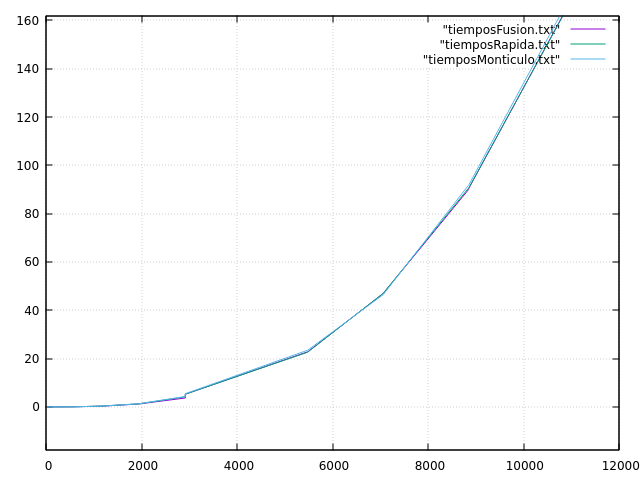
\includegraphics[width=0.7\linewidth]{./grafica}
\caption{Tiempos}
\label{fig:grafica}
\end{figure}
